%!TEX root = ../document.tex
\chapter{Grundlagen} \label{chp:Grundlagen}  
Im ersten Abschnitt wird der Microblogging-Dienst Twitter und seine Funktionen vorgestellt.
Danach werden geografische Begriffe und Verfahren eingeführt.

\todo{Einleitung schreiben}  

	\section{Der Microblogging-Dienst Twitter} 
	
		Zunächst wird definiert, welchen Dienst Twitter anbietet. 
		Danach wird ein geschichtlicher Überblick gegeben und einige Funktionen von Twitter erläutert.
		Zum Schluss wird aufgezeigt, welche Informationen in einem Tweet übermittelt werden.

		\subsection{Was ist Twitter?}
		
			Twitter wird als Kurznachrichten-Dienst, Microblogging-Dienst oder auch als Soziales-Netzwerk bezeichnet. 

			Twitter Geschäftsführer Kevin Thau hat 2010 auf dem Nokia-World-Congress öffentlich bestritten, dass Twitter ein Soziales-Netzwerk ist. 
			Laut Thau handelt es sich um ein Nachrichten-, Inhalts- und Informations-Netzwerk. 
			Er begründete dies damit, dass Twitter die Art und Weise wie Nachrichten verbreitet werden, geändert hat.
			Thaus Meinung nach kann praktisch jeder durch Twitter zum Journalisten werden kann. 
			Als Beispiel nennt er die Landung des Fluges 1549 auf dem Hudson River. 
			Die Augenzeugen hätten damals keine Mails versendet, um die Nachricht zu verbreiten, sondern die Nachricht via Twitter weitergegeben.
			Es lassen sich eine Reihe weiterer Beispiele derselben Art finden. 

			In \cite{Petrovic2013} wird ein Vergleich zwischen sogenannten Newswire anbietern und Twitter gezogen. \footnote{Newswire stellt eine Art Nachrichtenaggregator dar, über welchen Nachrichten aus verscheidenen Quellen aggregiert und weitergegeben werden. In Deutschland kommt die Deutsche Presseagentur diesem Konzept am nächsten.}
			Petrovic et al. fanden heraus, dass nahezu über alle Nachrichten, welche in den Newswires verbreitet wurden, auch im Twitter-Netzwerk berichtet wird.
			Nachrichten zu bestimmten, vermutlich sehr speziellen Themen oder Auslandsnachrichten, wurden ausschließlich in Twitter gefunden. 
			Diese Erkenntnisse decken sich mit der Einschätzung von Kevin Thau.

			In \cite{Kwak2010} wird die Einschätzung, bei Twitter handele es sich nicht um ein soziales Netzwerk, wissenschaftlich bestätigt.
			Kwak et al überprüfen die in \cite{Newman2003} beschriebenen Eigenschaften sozialer Netzwerke und kommen zu dem Schluss, dass Twitter diese Eigenschaften nicht erfüllt.	

			Die Bezeichnung Kurznachrichten-Dienst ist irreführend, da dieser mit sms \footnote{small messeneger service} in Verbindung gebracht werden kann. 
			Tatsächlich galt der sms in der Anfangsphase von Twitter als Vorbild für den Dienst.
			In Twitter werden Nachrichten allerdings standardmäßig allen Benutzern zur Verfügung gestellt und können eingesehen werden. 
			Des weiteren wird eine Liste der Nachrichten, die von einem Nutzer verfasst wurden, als Liste in umgekehrter chronologischer Reihenfolge auf dessen Profil dargestellt.
			Damit ähnelt das Twitter-Profil einem Blog mit Einträgen, deren Länge 140 Zeichen nicht überschreiten darf. 
			Die Darstellung als Liste, und die Funktion einen Tweet standardmäßig allen Nutzern freizugeben, unterscheidet sich grundlegend von der Funktion des sms.
			Beim sms wird eine Nachricht direkt an einen Empfänger gesendet und nicht öffentlich verbreitet.
			Im sms steht die Konversation zweier Nutzer im Vordergrund, wohingegen Nachrichten im Twitter-Netzwerk einen Broadcast an alle Nutzer darstellen.

			Die 140 Zeichen langen Nachrichten in Twitter werden als Tweets bezeichnet.
			Tweet bedeutet übersetzt "'Zwitschern"', womit die Redenwendung '"Die Spatzen zwitschern es von den Dächern"' auch im Twitter-Netzwerk zu einer passenden Redewendung wird.  
			Aufgrund der Erkenntnisse von \cite{Kwak2010} und der schlüssigen Argumentation von Kevin Thau ist es naheliegend, Twitter als Microblogging-Dienst zu bezeichnen.

		\subsection{Geschichtliches}
			
			Twitter wurde 2006 von Jack Dorsey, Biz Stone, Noah Glass und Evan Williams gegründet.
			Ursprünglich war Twitter zur internen Kommunikation innerhalb der Firma Odeo geplant.
			Schnell wurde allerdings klar, dass in dem Dienst mehr Potenzial steckt und so wurde Twitter öffentlich gemacht.
			Seitdem erfreut sich der Dienst einer wachsenden Nutzer-Gemeinde.
			Die Twitter-Gründer haben von Anfang an keine exakten Nutzer-Zahlen oder die Anzahl der versendeten Twitter-Kurznachrichten bekanntgegeben.
			Die Gründer sind davon überzeugt, dass anhand der reinen Nutzer-Zahlen und gesendeten Twitter-Kurznachrichten nicht die "'Gesundheit"' des Twitter-Netzwerks nachvollzogen werden.
			Andererseits werden durch diese Maßnahme auch strategische Ziele verfolgt.  \footnote{http://www.pbs.org/mediashift/2007/05/twitter-founders-thrive-on-micro-blogging-constraints137}
			2013 ging Twitter an die Börse und vermeldete 100 Millionen täglich aktive Nutzer und über 500 Millionen Twitter-Kurznachrichten, die täglich über den Dienst versendet werden. 

		\subsection{Funktionen von Twitter}
			
			Der Mikroblogging-Dienst Twitter bietet neben dem Profil, auf dem die Tweets des Nutzers angezeigt werden, noch eine Reihe weiterer Funktionen. 
			Im folgenden soll das Twitter-Profil und die Timeline kurz erläutert werden. 
			Eine der zentralen Funktionen von Twitter ist das sogennante "'Folgen"'.
			Danach werden Funktionen wie das weitergeben eines Tweets, Favorisieren und Antworten erklärt. 
			Zum Schluss wird auf den gesendeten Tweet-Inhalt eingegangen.

			\begin{figure}[h!]
			\begin{center}
			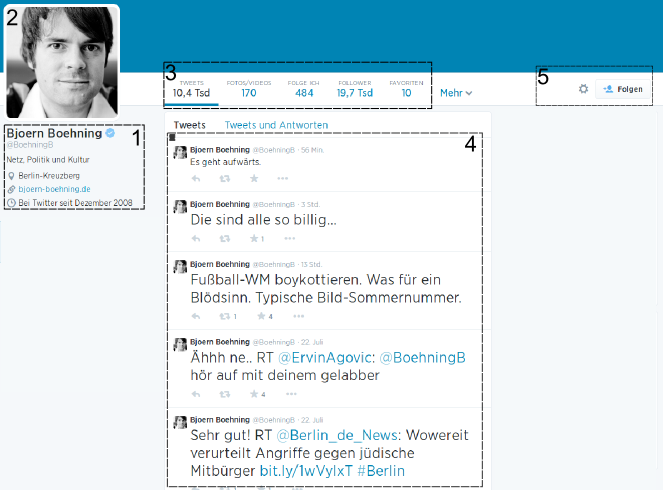
\includegraphics[scale=0.4]{profile.png}
			\caption{Die Tweet-Timeline}
			\label{img:twitterProfile}
			\end{center}
			\end{figure}	


			\paragraph{Das Nutzer-Profil und die Nutzer-Timeline}
				Das Nutzer-Profil kann über die Url http://twitter.com/BENUTZERNAME abgerufen werden und bietet neben der Nutzer-Timeline, in der die Tweets des Nutzers angezeigt werden, eine Reihe an weiteren Informationen.
				In Abbildung \ref{img:twitterProfile} ist in der Mitte die Timeline des Benutzers dargestellt, in der die Tweets zu sehen sind. 
				Folgende Bereiche können unterschieden werden.
				\begin{enumerate}
					\item Nutzername und Informationen über den Nutzer. 
					\item Profilbild
					\item Allgemeine Informationen über den Benutzer und dessen Netzwerk
					\item Nutzer-Timeline: Tweets des Nutzers in umgekehrter chronologischer Reihenfolge 
					\item Button zum Folgen
				\end{enumerate}
				
				Unter dem Profilbild links sind Informationen des Nutzers aufgelistet.
				Diese Informationen kann der Nutzer selbst einstellen.   

			\paragraph{Folgen (Following/Follower)}
				
				Diese Funktion erlaubt es Tweets eines bestimmten Nutzers zu abonnieren. 
				Im Twitter-Umfeld spricht man von "'following"' oder "'folgen"', wenn man die Tweets eines bestimmten Nutzers abonniert.
				Hat man Tweets eines bestimmten Nutzers abonniert, so wird man als dessen "'Follower"' bezeichnet. 
				Das englische Wort "'Follower"' hat sich im Twitter-Umfeld und auch im deutschsprachigen Raum etabliert. 
				Auch auf der Twitter Website wird '"Follower"' nicht ins deutsche übersetzt.
				In der vorliegenden Arbeit wird ebenfalls auf eine Übersetzung verzichtet. 

				In Abbildung \ref{img:twitterProfile} an Position 3 wird unter '"Folge ich"' die Anzahl der Twitter-Nutzer angezeigt, denen der Beispielnutzer folgt. 
				Neben dem Feld '"Folge ich"' wird unter '"Follower"' angezeigt, wieviele Nutzer dem Beispielnutzer folgen.

			\paragraph{Persönliche Timeline}
				Jeder Twitter-Nutzer hat seine persönliche "'Timeline"'.
				In dieser werden die Tweets derjenigen Nutzer angezeigt, denen er folgt. 
				Die "'Timeline"' kann als Aggregation von Tweets betrachtet werden.
				Diese "'Timeline"' ist die zentrale Stelle, an der ein Twitte-Nutzer Tweets anderer Nutzer empfangen und lesen kann.
				Auch hier werden die Tweets in umgekehrter chronologischer Reihenfolge angezeigt.  

			\paragraph{Weiterleiten eines Tweets (Retweet)}

				Unter einem "'Retweet"' versteht man das Weiterleiten eines Tweets, den man nicht selbst verfasst hat.
				Genauer gesagt wird der Tweet übernommen und ein Hinweis hinzugefügt, dass es sich um einen sogenannten "'Retweet"' handelt.
				Es wird damit gekennzeichnet, dass dieser Tweet nicht von dem Nutzer selbst verfasst wurde.
				Diese Funktion wird hauptsächlich genutzt, um Nachrichten schnell zu verbreiten, ohne diese neu eingeben zu müssen. 
				Die Weitergabe an die eigenen Follower impliziert einen gewissen Grad an Kontrolle und Filterfunktion. 
				Der weitergebende Nutzer kontrolliert und filtert die Nachrichten, die er erhält.
				Ein Nutzer gibt nur diejenigen Tweets weiter, denen er eine Gewisse Relevanz beimisst.
				Oder von denen er erwartet, dass sie seine Follower interessieren könnten. 
				Mit dieser Funktion können einzelne Nutzer eine Art Filterfunktion übernehmen, welche früher Journalisten vorbehalten war. 
				Es darf jedoch nicht vergessen werden, dass der Nutzer nur im Rahmen seiner eigenen Möglichkeiten einen Tweet verifizieren kann.
				Nachrichten in Twitter stellen keinesfalls gesicherte Fakten dar.
				Auch eine große Verbreitung durch viele Retweets ändert daran nichts.
				Durch diese Funktion können Nutzer zu Tweet-Aggregatoren werden.
				Der Nutzer abonniert viele Nutzer, aber gibt nur relevante oder themenspezifische Tweets an seine Follower weiter. 

		\subsection{Die Twitter Streaming API}

			Die Twitter Streaming API \footnote{Application Programming Interface} ermöglicht es, Tweets programmatisch abzurufen.
			Dabei wird von Twitter ein Sample aller aktuell erstellten Tweets zur Verfügung gestellt.  
			Das Sample beinhaltet maximal 1\% aller aktuell erstellten Tweets.
			Die Streaming API ermöglicht es ebenfalls, nach bestimmten Eigenschaften der Tweets zu suchen.
			Beispielsweise lassen sich bestimmte Stichworte angeben, anhand derer die Ergebnisse gefiltert werden sollen.
			Es können auch ausschließlich Tweets abgefragt werden, welche eine Georeferenz in Form von Längen- und Breitengrad aufweisen. 

			Durch eine programmatische Abfrage an die Streaming Api können automatisiert große Datensätze zu Analysezwecken erstellt werden. 

		\subsection{Daten einer Twitter-Nachricht} \label{sub:DatenInTwitterNachricht} 
			
			Neben den direkt sichtbaren Informationen enthält ein Tweet eine Reihe weiterer Daten.
			Betrachtet man einen einzelnen Tweet, beispielsweise auf twitter.com erscheint dieser wie in Abbildung \ref{img:tweet}.

			\begin{enumerate}
				\item Profilbild des Verfassers
				\item Name, Benutzername und Zeit
				\item Der Tweet-Text
			\end{enumerate}


			\begin{figure}[h!]
			\begin{center}
			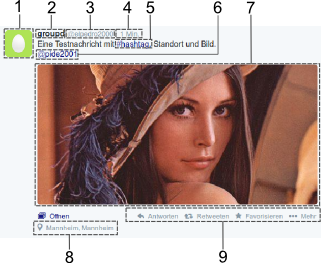
\includegraphics[scale=0.8]{tweet.pdf}
			\caption{Ein Tweet}
			\label{img:tweet}
			\end{center}
			\end{figure}	


			Erfasst man einen Tweet allerdings über die Streaming API, wird eine Reihe weiterer Daten mitgeliefert.
			Mit jedem Tweet werden auch Daten aus dem Twitter-Profil des Verfassers versendet.
			Es werden im folgenden der Nutzer-Standort, die Nutzer-Zeitzone und die geografischen Koordinaten betrachtet.

			\paragraph{Geografische Koordinaten}
				
				In den Tweet-Daten können geografische Koordinaten in Form von Längen- und Breitengrad angegeben sein. 
				Diese Koordinaten zeigen an, wo sich der Verfasser befand als er den Tweet abgesetzt hat.
				Wenn diese Koordinaten angegeben sind hat der Nutzer explizit zugestimmt, dass die Koordinaten seines aktuellen Aufenthaltsortes dem Tweet angehängt werden. 
				Die Bestimmung der Koordinaten erfolgt über ein GPS-Modul in einem Smartphone oder mit Hilfe von GeoIp an einem PC.
				Das Anhängen der Koordinaten an einen Tweet wird vollautomatisch durch das Programm übernommen, mit welchem der Tweet verfasst wurde.

			\paragraph{Nutzer-Standort} 
				
				Der Nutzer-Standort wird vom Benutzer in den Profil Einstellungen eingegeben.
				In Abbildung \ref{img:twitterLocation} ist der Dialog zur Nutzer-Standort Eingabe in den Twitter-Profil Einstellungen abgebildet.


				\begin{figure}[!ht]
						\begin{center}
							
\includegraphics[scale=0.5]{twitterUL.png}
							\caption{Eingabe des Nutzer-Standortes}
							\label{img:twitterLocation}
						\end{center}
					\end{figure}	
				%Quelle: http://www.twitter.com

				Der Nutzer-Standort wird direkt übernommen und unterliegt keiner weiteren Verarbeitung seitens Twitter.
				Dies bedeutet der Nutzer-Standort wird übernommen, wie er vom Nutzer eingegeben wird.
				Das Dialogfeld ist lediglich auf ein Maximum von 30 Zeichen beschränkt. 

			\paragraph{Nutzer-Zeitzone} 

				Die Nutzer-Zeitzone kann vom Benutzer in den Profil Einstellungen aus einer Liste gewählt werden.
				Der Datenwert der Nutzer-Zeitzone stellt also garantiert eine Zeitzone dar. 
				In Abbildung \ref{img:twitterTZ} ist der Auswahldialog in den Twitter-Profil Einstellungen zu sehen.

				\begin{figure}[!ht]
					\begin{center}
						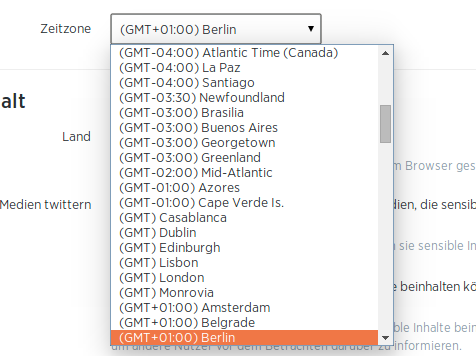
\includegraphics[scale=0.5]{tz.png}
						\caption{Zeitzonen Auswahldialog}
						\label{img:twitterTZ}
					\end{center}
				\end{figure}	
				%Quelle: http://www.twitter.com

				Es wird nicht geprüft, ob der Nutzer sich auch in dieser Zeitzone befindet.
				Der Nutzer könnte eine bewusste Fehleingabe machen oder aber die Zeitzone nicht wählen.
				Der Standardwert der Nutzer-Zeitzone ist dann "'Pacific Time (US and Canada)"'.

	\section{Geografische Grundlagen und Begriffe}
	
		In diesem Kapitel sollen geografische Grundbegriffe erläutert werden. 
		Einige geografische Begriffe werden in verschiedenen wissenschaftlichen Bereichen unterschiedlich genutzt und teilweise widersprüchlich definiert. 
		Um Missverständnissen vorzubeugen, wird hier definiert, was in der vorliegenden Arbeit unter den einzelnen Begriffen zu verstehen ist.
		Eine Reihe von Begriffen wird selbst definiert, um bestimmte Sachverhalte im Kontext dieser Arbeit klarer ausdrücken zu können. 

		\subsection{Geografische Koordinaten} 

			Eine Position auf dem Globus wird mit zwei Werten beschrieben, dem sogenannten Längengrad und dem sogenannten Breitengrad.
			Diese beiden Werte werden als geografische Koordinaten bezeichnet. 
			Mit diesen zwei Werten und einem geodätischen Referenzsystemsystem kann die Position auf dem Globus exakt bestimmt werden.  
			Die geografischen Angaben in Twitter liegen bezüglich des geodätischen Referenzsystems WGS84 vor und sind nur für dieses gültig.
			Werden diese bezüglich eines anderen geodätischen Referenzsystems ausgewertet ist die Position auf dem Globus nicht korrekt.
			Es ist dann eine Transformation der Werte erforderlich.
			Heutzutage ist das Referenzsystem WGS84 weit verbreitet.

			Ein geodätisches Referenzsystem besteht aus einem kartesischen Rechtssystem mit definierter Lage und Ausrichtung, einem Referenzellipsoid und einer Festlegung zur Messung der Winkel.

			Die Lage und Ausrichtung des kartesische Rechtssystems erfolgt relativ zur Erde. 
			Der Ursprung des Koordinatensystems liegt im Zentrum des Globus.
			Die Z-Achse zeigt dabei in Richtung Nordpol und die X-Achse in Richtung 0 Grad Länge (Nullmeridian) und 0 Grad Breite (Äquator). 
			Mit diesen zwei Werten ist die Lage eines kartesischen Rechtssystem eindeutig definiert.
			In Abbildung \ref{img:lnglat} sind sowohl die Lage des Nullmeridian und des Äquators sowie die Lage des kartesischen Referenzsystems dargestellt. 

			In diesem Koordinatensystem sind zusätzlich Referenzpunkte festgelegt.
			Diese Referenzpunkte werden benötigt, um einen Referenzellipsoid zu verankern. 
			Auf diesem Ellipsoid sind ebenfalls definierte Referenzpunkte festgelegt, die mit den Referenzpunkten im Koordinatensystem zur Deckung gebracht werden.
			Der Referenzellipsoid soll eine möglichst genaue Approximation der Erde darstellen und diese im geodätischen Referenzsystem repräsentieren. 
			Ein Punkt auf diesem Ellipsoid entspricht damit einem Punkt auf der Erde.

			Mit diesen Komponenten kann nun ein Punkt auf dem Ellipsoid eindeutig bestimmt werden.
			Der Längen- und Breitengrad eines Punktes P auf dem Ellipsoid lässt sich folgendermaßen bestimmen:

			Durch den Punkt P auf dem Ellipsoid und den Ursprung z des Koordinatensystems wird eine Gerade g gezogen. 
			Der Wert für den Breitengrad ist nun der Winkel $\phi$ zwischen g und der Äquatorebene.
			Nun wird der Punkt P auf einen Punkt Q auf der Äquatorebene projiziert.
			Zwischen z und dem projizierten Punkt Q kann nun wiederum eine Gerade h gezogen werden.
			Der Wert für den Längengrad ist der Winkel $\lambda$ zwischen der X-Achse und der Gerade h (Abbildung \ref{img:lnglat}).
			\footnote{Vergleiche Geoinformatik Lexikon der Universität Rostock (abgerufen Juli 2014): http://www.geoinformatik.uni-rostock.de/lexikon.asp \\ Vorlesungen zur Geo-Informatik von Prof. Dr.-Ing. Ralf Bill (abgerufen Juli 2014): http://www.geoinformatik.uni-rostock.de/vorlesungsthem.asp \label{ft:geoinfolex}  Juli 2014}



			\begin{figure}[h!]
			\begin{center}
				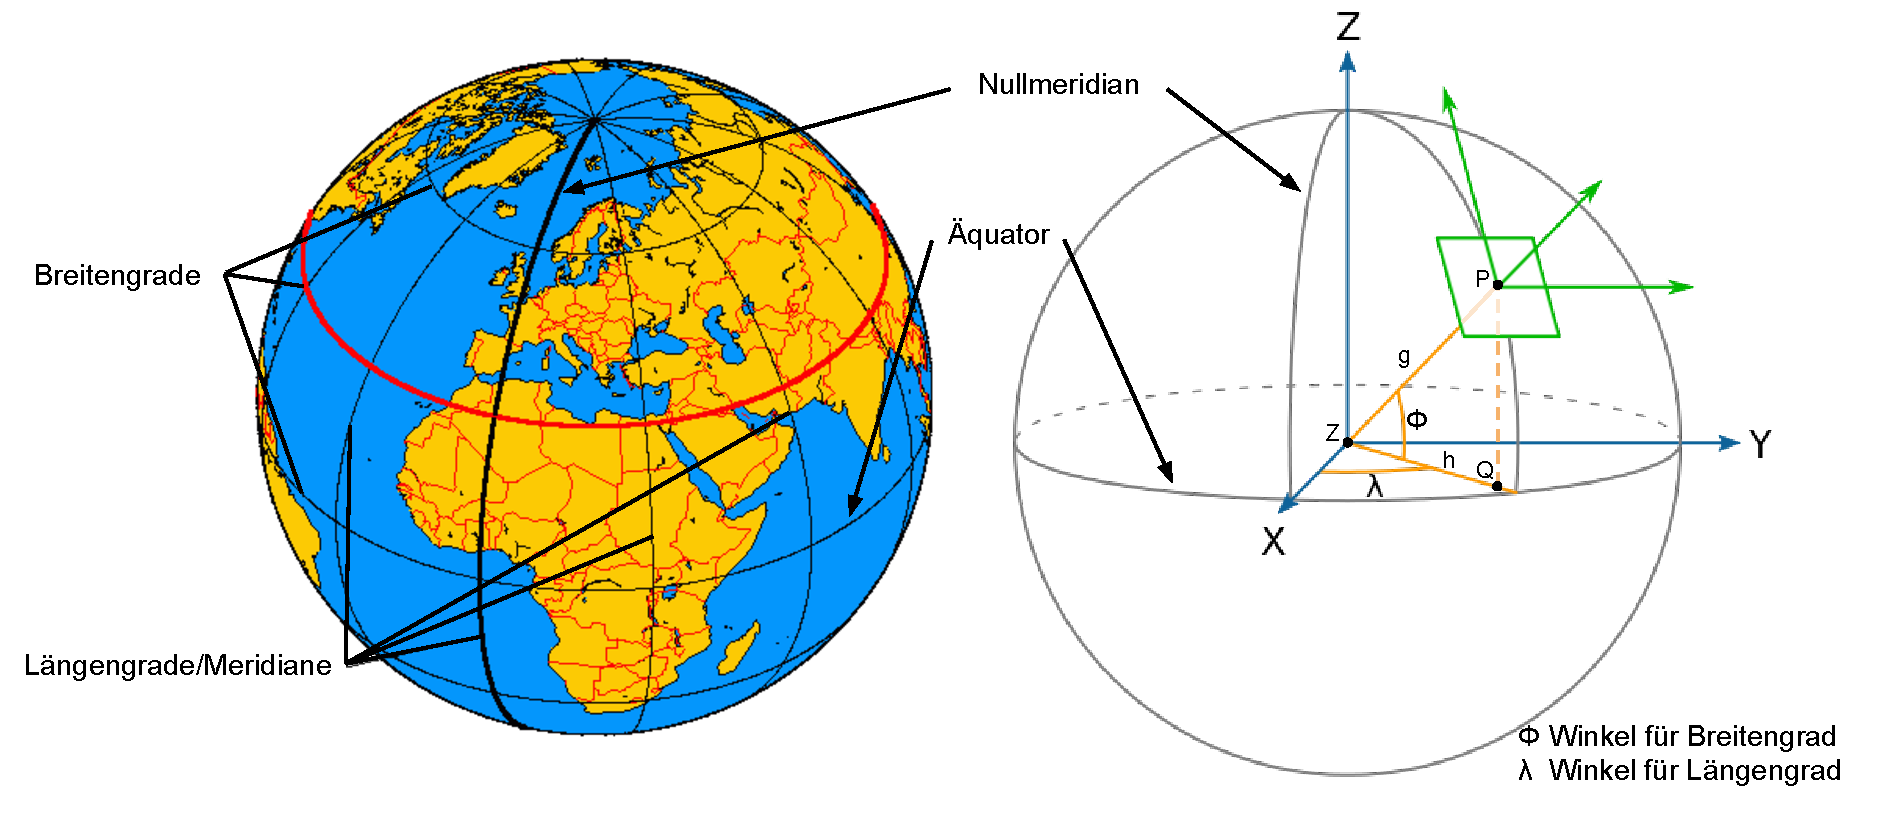
\includegraphics[scale=0.5]{globuseMitLngLat.pdf}
				\caption{Nullmeridian und Äquator (linke Bildseiten);Lage des kartesischen Rechtssystems(rechte Bildseite)}
				\label{img:lnglat}
			\end{center}
			\end{figure}	
			\todo{Referenzen Bild} 
			%vgl. http://de.wikipedia.org/wiki/Meridian_(Geographie)#mediaviewer/Datei:Meridian-International.PNG
			%vgl. http://en.wikipedia.org/wiki/Geodetic_datum#mediaviewer/File:ECEF_ENU_Longitude_Latitude_relationships.svg

		\subsection{Georeferenz} 
			
			Ist einem Datensatz, einem Datum oder einem Objekt eine geografische Lage oder Position zugeordnet, so wird diese als Georeferenz (auch Raumbezug genannt) bezeichnet.
			Eine Georeferenz kann auf verschiedene Arten und mit unterschiedlicher Genauigkeit angegeben werden.
			Dies hängt von den Anforderungen ab, die an die Georeferenz gestellt werden. 
			Beispielsweise stellen die in Kapitel \ref{chp:Einleitung} erwähnten Anwendungen unterschiedliche Anforderungen an die Genauigkeit der Georeferenz. \footref{ft:geoinfolex} 
			
			Die Georeferenz lässt sich bezüglich der Genauigkeit weiter unterteilen in: 
		
			\begin{description}

	 			\item[Direkte Georeferenz (Direkter Raumbezug)] 
	 				
	 				Unter einer direkten Georeferenz versteht man die Angabe einer konkreten Koordinate bezüglich eines geeigneten geodätischen Referenzsystems. \footref{ft:geoinfolex} 

	 			\item[Indirekte Georeferenz (Indirekter Raumbezug)] 
	 				
	 				Unter indirektem Raumbezug werden alle Angaben verstanden, die eine ungenaue Position bezüglich eines beliebigen Referenzysystems bestimmen.
		 			Ungenau ist in dem Sinne zu verstehen, dass die Angabe der Position auch eine Fläche beschreiben kann.
		 			Zusätzlich muss das gewählte Referenzsystem nicht zwingenderweise unveränderlich sein.   
		 			Beispiele für die Angabe eines indirekten Raumbezugs wären Länder, Adressen, Postleitzahlen oder auch Telefonvorwahlen. 
		 			Alle diese Angaben, mit Ausnahme der Adresse, definieren eine geografische Fläche. 
		 			Diese Fläche ist nicht zwingenderweise klar abzugrenzen. \footref{ft:geoinfolex} 

			\end{description}

		\subsection{Geografische Objekte}
			
			Ein geografisches Objekt ist ein Objekt der Realwelt dessen Position durch eine Georeferenz bestimmt werden kann. 
			Die EN ISO 19110:2005 Norm beschreibt ein geografisches Objekt folgendermaßen: 

			"'Geografische Objekte sind Erscheinungen der realen Welt, die einen Bezug zur Erde (Raumbezug) haben..."' \cite{ISO19110:2005}.

			Es wird insbesondere nicht festgelegt, ob es sich dabei um eine direkte oder eine indirekte Georeferenz handelt.
			Beispiele für geografische Objekte sind: Städte, Länder, Häuser oder auch Fahrzeuge.
			Insbesondere sind auch Menschen geographische Objekte, da sie zu jeder Zeit einen Bezug zur Erde haben.

		\subsection{Geografische Position}
		
			Unter einer geografischen Position wird in dieser Arbeit eine Position auf dem Globus verstanden, die durch geografische Koordinaten bestimmt.

		\subsection{Toponyme}  
			
			Im Deutschen werden Eigennamen für geografische Objekte als Ortsnamen bezeichnet. 
			Dies ist insofern missverständlich, da Ortsnamen nicht nur Namen für Orte im Sinne von Ortschaften sind, sondern auch Namen für andere geografische Objekte.
			In der vorliegenden Arbeit wird deshalb der Begriff Toponym verwendet. 

		\subsection{Zuordnung von Toponymen zu geografischen Objekten} \label{sec:zuordnungToponymeGeogObj}

			Wird ein Toponym als Angabe für eine geografische Position verwendet, muss dieses einem konkreten geografischen Objekt zugeordnet werden. 
			Die Zuordnung von Toponymen zu geografischen Objekten kann allerdings problematisch sein.
			In Woodruff et al. \cite{Woodruff1994} wird auf die Probleme bei der Zuordnung von Toponymen zu geografischen Objekten eingegangen.
			Es lassen sich daraus folgende Hauptproblemfelder ableiten:

			\begin{description}

				\item[Mehrdeutigkeiten von Toponymen]

					Toponyme sind oft doppel- oder mehrdeutig und verweisen somit auf mehrere geografische Objekte.
				
					Es gibt zahlreiche Städte-Namen, die in mehreren Ländern verwendet werden.
					Ein gutes Beispiel hierfür sind US-Städte. 
					In Tabelle \ref{tab:usCitiesGermanNames} sind einige Städte-Namen und die Vorkommen in den USA aufgelistet.
					
					\begin{table}[htpb]
						\caption{Häufige deutsche Städtenamen in den USA} 
						\centering
						\begin{tabular}{|c|c|}
							\hline
							Name & Anzahl in den USA \\
							\hline\hline
							Hannover & 40 \\
							\hline
							Berlin & 39 \\
							\hline
							Hamburg & 30 \\
							\hline
						\end{tabular}
						\label{tab:usCitiesGermanNames} 
					\end{table}
					%QUELLE ??? 

					Diese Mehrdeutigkeiten stellen ein Problem dar, da ohne zusätzliche Informationen nicht mit Sicherheit bestimmt werden kann, welches geografische Objekt gemeint ist.
					
				\item [Verschiedene Schreibweisen]

					Zu einem Toponyme können verschiedene Schreibweisen existieren. 
					Dies kann beispielsweise durch die verwendete Sprache bedingt sein.
					Im Englischen wird für München auch Munich verwendet.
					Es kann aber auch zu alternativen Schreibweisen durch die Verwendung eines Alphabets kommen, welches nicht den benötigten Zeichensatz zur Verfügung stellt.
					Existiert beispielsweise in einem Alphabet kein "'ü"', würde München als Muenchen geschrieben.  

			  	\item [Alternative Toponyme]

			  		Woodruff et al. beschreiben das Problem der Neologismen bei Toponymen. 
			  		Mit Neologismen werden Wortneuschöpfungen in Sprachgemeinschaften bezeichnet, die zunächst nicht allgemein bekannt sind. 
			  		Dies kann auf Namen geografischer Objekte derart übertragen werden, dass für geografische Objekte lokal begrenzte oder in einem gewissen Kontext gebräuchliche Toponyme verwendet werden.

			  		Als Beispiel sollen hier alternative Toponyme in Form von Bei- und Spitznamen für Städte dienen.
					Neben den offiziellen Namen für Städte kann eine Reihe von alternativen Toponymen existieren.
					In Wikipedia sind für die Stadt Detroit, im US-Bundesstaat Michigan, folgende Beinamen angegeben: 

					 "'The Motor City"', "'Motown"', "'Hockeytown"', "'Rock City"', "'The D"'.

					Die ersten zwei dürften weltweit einen gewissen Bekanntheitsgrad haben. 
					"'Hockeytown"', "'Rock City"' und "'The D"' dürften allerdings weniger bekannt sein.
					Es ist deshalb schwer, diesen Toponymen ein geografisches Objekt zuzuordnen oder diese überhaupt als Toponym zu identifizieren.

			\end{description}  

		\subsection{Geografische Region} 
			
			Unter einer geografischen Region werden hier Flächen auf dem Globus verstanden.
			Diese können nicht durch einen einzelnen Punkt beschrieben werden. 
			Flächen werden üblicherweise durch ein Polygon beschrieben. 
			Das Polygon wird durch eine Menge geografischer Positionen bestimmt.
			Diese werden in einer festgelegten Reihenfolge durch eine Linie verbunden.

			Bundesländer oder Länder sind Beispiele für geografische Regionen.
			
		\subsection{Geografischer Bezug} 

			Kann einem Datenwert in irgendeiner Weise eine Georeferenz zugeordnet werden, hat dieser Datenwert geografischen Bezug.
			Datenwerte mit geografischem Bezug können weiter unterteilt werden in Datenwerte mit unmittelbarem geografischen Bezug oder mittelbarem geografischen Bezug. 

			\begin{description}
				\item[Datenwerte mit unmittelbarem geografischem Bezug]

					Einem Datenwert mit unmittelbarem geografischen Bezug lässt sich durch die in ihm enthaltene Information eine Georeferenz zuweisen.	

					Beispielsweise haben Zeitzonen unmittelbaren geografischen Bezug, da die in ihnen enthaltene Information unmittelbar einer Georeferenz zugewiesen werden kann.
					Auch Toponyme, die eindeutig sind, haben unmittelbaren geografischen Bezug.

				\item[Werte mit mittelbarem geografischem Bezug] 

					Ein Wert hat genau dann mittelbaren geografischen Bezug, wenn die in ihm enthaltene Information nicht direkt auf ein geografisches Objekt verweist, ihm aber trotzdem eine Georeferenz zugeordnet werden kann.
					Dabei ist die eigentliche Information des Wertes unerheblich. 
					Der geografische Bezug erfolgt beispielsweise durch die geografisch begrenzte Verwendung des Wertes. 

					Dies soll an einem Beispiel erläutert werden:\\
					Die folgenden drei Datenwerte werden betrachtet.

					\begin{enumerate}
					 	\item Äbierra
					 	\item Grumbeer
					 	\item Tüfte 
					 \end{enumerate} 

					Die drei Begriffe bezeichnen ein Gemüse, genauer Kartoffeln.
					Die Datenwerte bezeichnen also insbesondere kein geografisches Objekt und haben somit keinen unmittelbaren geografischen Bezug.
					Jeder dieser Bezeichnungen stammt aber aus unterschiedlichen Regionen Deutschlands, denn es handelt sich um dialektische Begriffe.
					Äbierra wird in Baden-Württemberg, Grumbeer in der Pfalz und Tüfte in Norddeutschland verwendet.
					Durch ihre geografisch begrenzte Verwendung können sie damit einer geografischen Region zugeordnet werden.
					Durch diese Datenwerte kann also auf eine Region Deutschlands geschlossen werden und somit auf ein geografisches Objekt.

			\end{description}

		\subsection{Geografische Indikatoren}

			Liefert ein Datensatz Informationen zu einem Objekt, dessen Georeferenz unbekannt ist, kann aus diesen Daten möglicherweise eine Georeferenz abgeleitet werden. 
			Dies ist genau dann der Fall, wenn in dem Datensatz Datenwerte enthalten sind, die mittelbaren oder unmittelbaren geografischen Bezug aufweisen.
			Diese Datenwerte können als Hinweis auf die Georeferenz des Datensatzes genutzt werden.
			Diese werden hier als geografische Indikatoren bezeichnet.

			In Abbildung \ref{img:geogIndi} ist der Zusammenhang zwischen geografischen Indikatoren, geografischem Bezug, geografischem Objekt und einer Georeferenz dargestellt. 
			Das geografische Objekt A hat eine Georeferenz G.
			Der Datensatz A liefert Informationen zum geografischen Objekt A.
			Information a und Information b haben einen geografischen Bezug zu G und sind somit geografische Indikatoren.
			Ist zum geografischen Objekt A keine Georeferenz bekannt, so lässt sich durch die geografischen Indikatoren a und b die Georeferenz G ableiten. 

			\begin{figure}[h!]
			\begin{center}
				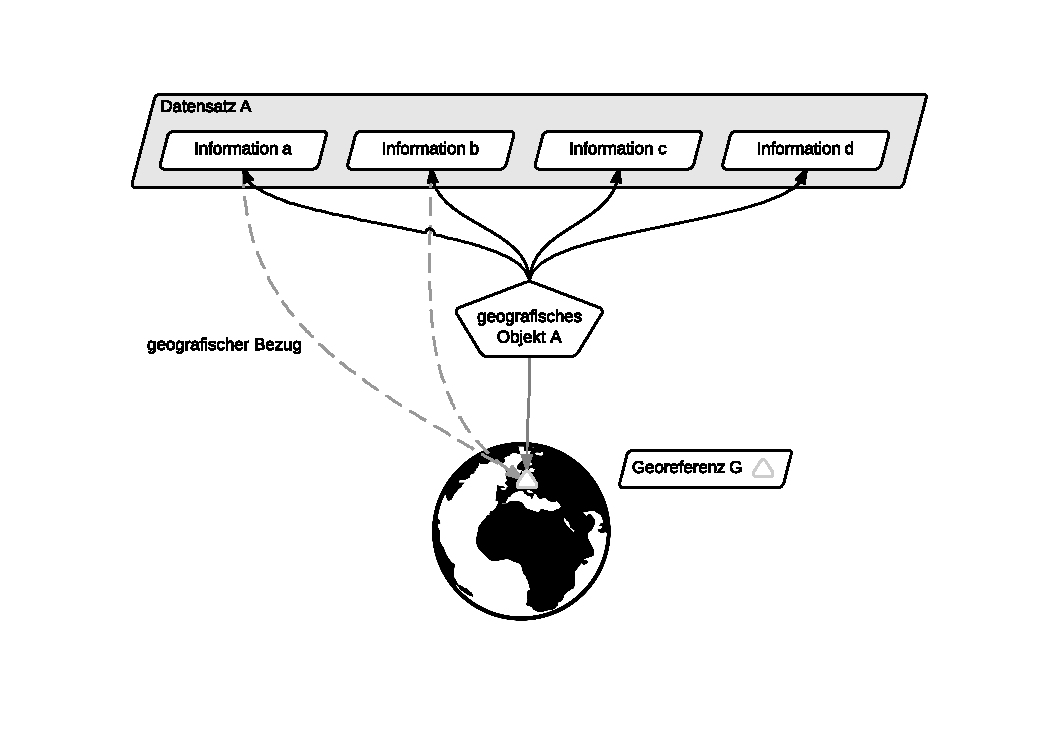
\includegraphics[scale=0.8]{geogIndikatoren.pdf}
				\caption{Geografische Indikatoren}
				\label{img:geogIndi}
			\end{center}
			\end{figure}	
			%Earth designed by Liane Thönnes from the thenounproject.com
			%Pin designed by Simple Icons from the thenounproject.com  

		\subsection{Geografische Hierarchie} \label{sub:geografischeHierarchie} 
			
			In der vorliegenden Arbeit wird eine geografische Hierarchie verwendet, um eine Einteilung der Erde in geografische Regionen umzusetzen.

			Eine Aufteilung der Erde in geografische Regionen lässt sich auf oberster Ebene mit Hilfe von Ländern und deren Grenzen umsetzen. 
			Die meisten Länder sind in weitere administrative Einheiten aufgeteilt.
			Diese geografischen Regionen werden hier als Verwaltungseinheiten bezeichnet.
			Es wird zwischen Verwaltungseinheiten erster und zweiter Ordnung unterschieden. 
			Der Vatikan-Staat und das Fürstentum Monaco sind dabei Ausnahmen.
			Beide werden aufgrund ihrer Größe nicht in weitere Verwaltungseinheiten unterteilt.
			In der untersten Ebene der Hierarchie werden schließlich Städte dargestellt.
			In der vorliegenden Arbeit wird das Ortsverzeichnis von geonames.org verwendet. 
			Dieses bildet die hier vorgestellte geografische Hierarchie ab.


			Wenn man als Beispiel Deutschland heranzieht, ergibt sich eine Einteilung wie in Abbildung \ref{img:hierarchy} dargestellt. \footnote{Aus Platzgründen sind im Bild pro Ebene nur einige wenige geografische Objekte aufgezählt.} 
			Die oberste Ebene beschreibt das Land worauf die zweite Ebene die Bundesländer darstellt.
			Auf der dritten Ebene werden die Regierungsbezirke abgebildet, worauf die Städte in der letzten Ebene folgen. 
			Analog kann die Einteilung für die USA vorgenommen werden, woraus sich die Hierarchie Country->State->County->City ergibt.
			Jedes Objekt einer Hierarchieebene beschreibt eine geografische Region. 
			Insbesondere besteht in einer solchen Hierarchie eine Teilmengenbeziehung zwischen den Ebenen. 
			Ein Objekt in einer Ebene liegt immer innerhalb der ihm übergeordneten Objekte.
			Insbesondere liegt die geografische Region die ein Objekt beschreibt komplett innerhalb des ihm übergeordneten Objekts.			

			\begin{figure}[h!]
			\begin{center}
			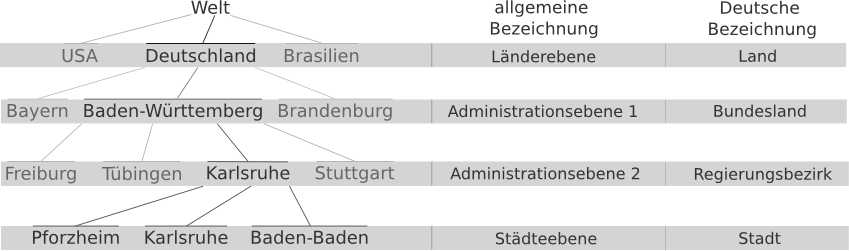
\includegraphics[scale=0.5]{hierarchie.png}
			\caption{Beispiel für geografische Hierarchieebenen}
			\label{img:hierarchy}
			\end{center}
			\end{figure}	

			In Abbildung \ref{img:globusHierarchie} ist die Einteilung des Globus in Länder und Verwaltungseinheiten dargestellt. 

			\begin{figure}[h!]
			\begin{center}
			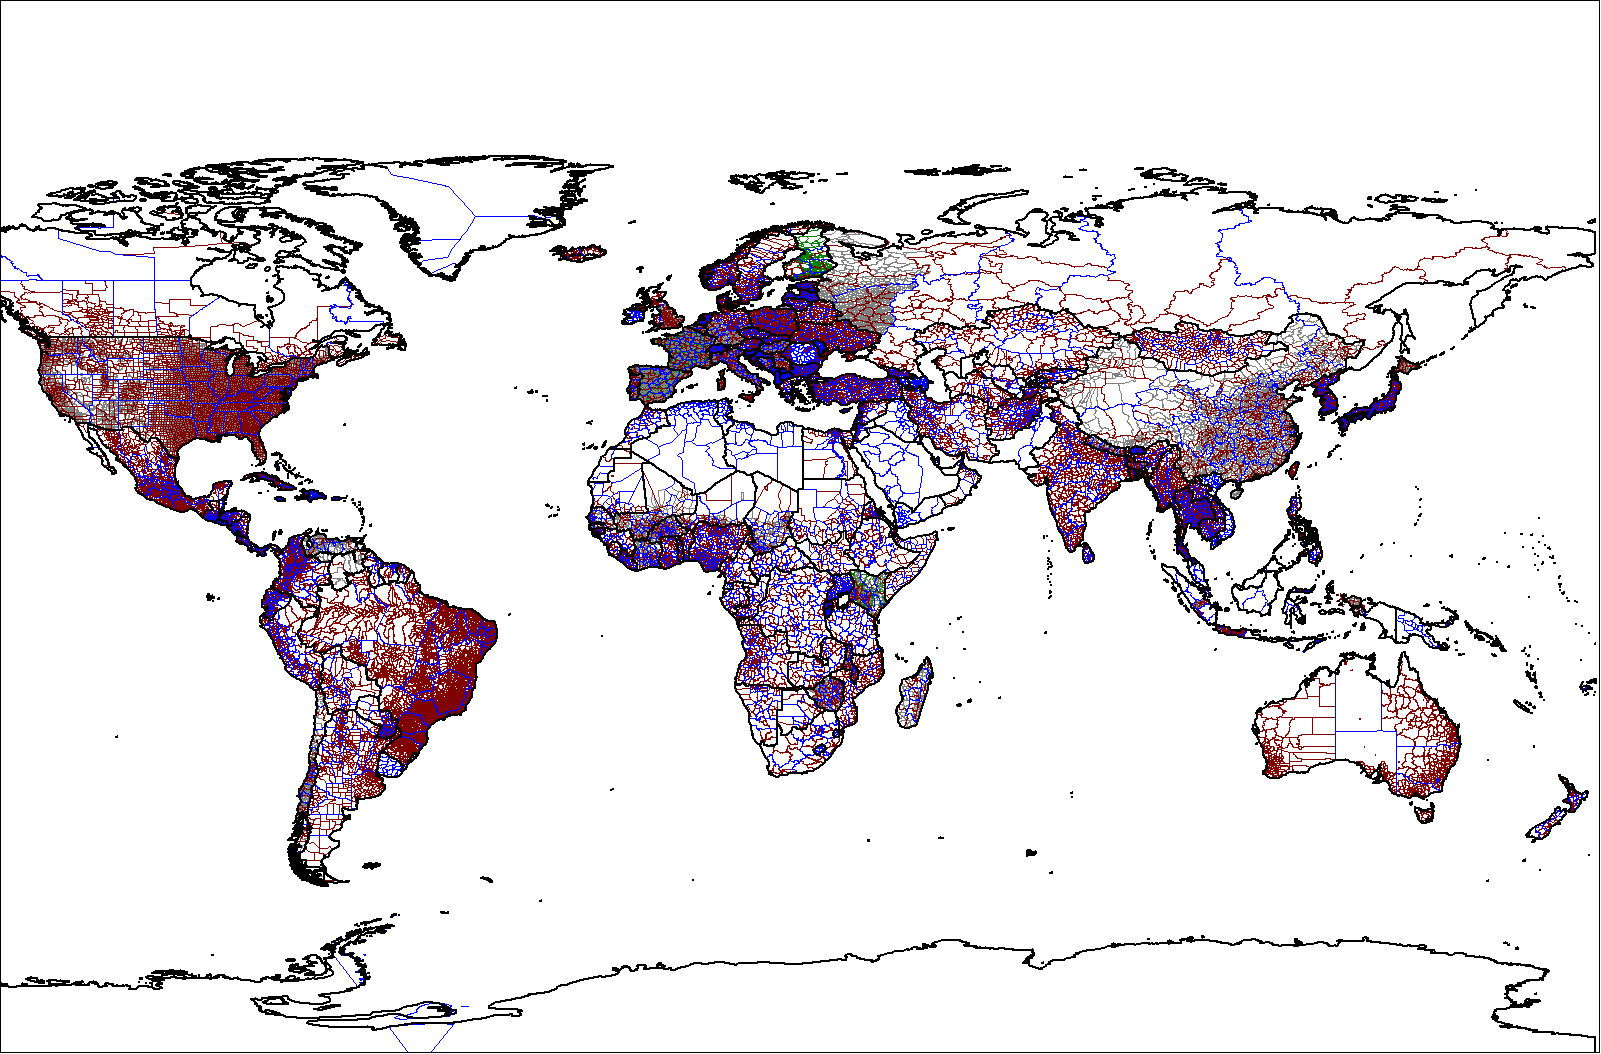
\includegraphics[scale=0.3]{globusHierarchie.png}
			\caption{Aufteilung der Welt in Verwaltungseinheiten}
			\label{img:globusHierarchie}
			\end{center}
			\end{figure}	
			%http://de.wikipedia.org/wiki/Verwaltungseinheit#mediaviewer/Datei:World_administrative_levels.png

		\subsection{Ortsverzeichnisse}

			In einem Ortsverzeichnis \footnote{Englisch: Gazetteer} sind Toponyme und deren zugehörige Georeferenzen gespeichert.
			Ortsverzeichnisse können sehr umfangreich sein und werden in Form einer Datenbank bereitgestellt.
			Meistens werden zu den Toponymen noch weitere Informationen hinterlegt.
			So bilden die Ortsverzeichnisse beispielsweise oft geografische Hierarchiebeziehungen ab.
			Aber auch Angaben zur Bevölkerungszahl oder die Angabe von alternativen Toponymen sind oft hinterlegt.

			Ortsverzeichnisse können genutzt werden, um Toponymen eine Georeferenz zuzuweisen. 
			Dabei wird ein gegebenes Toponym im Ortsverzeichnis nachgeschlagen, um die zugehörige Georeferenz zu erhalten.  
		
			Eines der bekanntesten Ortsverzeichnisse ist das frei erhältliche Ortsverzeichnis von geonames.org. 
			Dieses Ortsverzeichnis kann als CSV Datei\footnote{Comma Sperated Value} heruntergeladen werden.
			Neben umfangreichen Informationen wie Bevölkerungszahl, Sprache, Längen- und Breitengrad wird die geografische Hierarchie abgebildet.

			Die Daten von geonames.org werden aus diversen Quellen automatisch zusammengetragen. \footnote{Die genutzten Datenquellen können unter http://www.geonames.org/data-sources.html eingesehen werden} 
			Es werden allerdings auch Einträge von Nutzern erstellt. 
			Mittlerweile hat sich eine aktive Community rund um das Projekt entwickelt. 

			Das Ortsverzeichnis beinhaltet ca. 8,8 Millionen Toponyme und zugehörige Informationen. \footnote{Stand Dez. 2013, die Daten unterliegen ständiger Bearbeitung, die Anzahl der Einträge kann deshalb variieren} 
			Hinzu kommen ca. 8 Millionen alternative Toponyme.
			Geonames.org ist damit eine der umfangreichsten frei erhältlichen Ortsverzeichnisse.

			Jedem Toponym ist eine geografische Position in Form von Längen- und Breitengrad zugeordnet. 
			Es wird allerdings kein Polygon zur Beschreibung der geografischen Region angegeben.
			Durch die Teilmengen Beziehung, die in der geografischen Hierarchie abgebildet ist, können jedoch immer alle geografischen Hierarchieebenen bestimmt werden.

			In der vorliegenden Arbeit wird die geonames.org Datenbank mit Stand Dezember 2013 als Basis für geografische Informationen genutzt.
			Auch die verwendete geografische Hierarchie lässt sich aus der Datenbank gewinnen.

		

	

	
